Testiranja su obavljena na računalu s procesorom Intel Core i7 920 @ 2.66 GHz, s 6 GB RAM memorije i na operacijskom sustavu Windows 7. Razlog zašto testiranja nisu bila obavljena na Biolinuxu (ili nekoj drugoj Linux distribuciji) je taj što se Biolinux, na računalu koje se koristilo za testiranja, pokreće u virtualnom stroju, pa je upitno kako bi to utjecalo na performanse izvođenja samog programa. Za mjerenje vremena izvođenja korištena je metoda \textit{currentTimeMillis} razreda \textit{System}, dok je za mjerenje potrošnje memorije korišten alat \textit{Jprofiler}.

Za obavljanje testiranja korištena su tri tipa tekstualnih datoteka. Prvi tip tekstualnih datoteka se sastojao od nizova nukleotida i dodatnih znakova koji se još mogu pojaviti u takvim nizovima. Drugi tip tekstualnih datoteka sastojao se od nizova znakova koji predstavljaju proteine. Posljednji tip tekstualnih datoteka koje su korištene sastojale su se od nizova slučajno generiranih znakova iz osnovnog ASCII skupa znakova i to od znakova koji se mogu ispisati (dakle ne od specijalnih znakova). Prvi i drugi tip datoteka su preuzeti s \cite{corpus} te su ponešto prilagođene za obavljanje testiranja. Treći tip datoteka je bio generiran uz pomoć posebnog programa. Spomenute datoteke se razlikuju po tome koliko se različitih znakova može pojaviti u njima, odnosno koje su veličine abeceda iz kojih su te datoteke generirane. Tablica \ref{tbl:alphabetsize} prikazuje veličinu abeceda iz kojih su generirane određene datoteke, odnosno koliko najviše različitih znakova mogu sadržavati. 

\begin{table}[h]
\caption{Maksimalna veličina abecede pojedinih datoteka}
\label{tbl:alphabetsize}
\centering\begin{tabular}{c|c|c|c|}
 \hline
\multicolumn{1}{ |c| } {Vrsta niza} & Broj različitih znakova   \\ \hline
\multicolumn{1}{ |c| } {   DNK   }		&	15		\\ \hline
\multicolumn{1}{ |c| } {   Proteini   }	&	25		\\ \hline
\multicolumn{1}{ |c| } {   ASCII   }	&	95		\\ \hline
\end{tabular}
\end{table}


U ovom poglavlju pogledat ćemo performanse koje pruža implementirani FM-indeks i to u tri kategorije: brzina izgradnje, brzina obavljanja \textit{count} upita i memorijska potrošnja.

\section{Vrijeme izgradnje FM-indeksa}
Pogledajmo prvo performanse izgradnje FM-indeksa. Ovo je možda i jedan od najbitnijih faktora prilikom ocjene koliko je neka implementacija dobra, pošto je izgradnja samog indeksa računalno veoma zahtjevna operacija. Kako bi rezultati koji će biti prikazani u ovom poglavlju bili što relevantniji, vrijednosti koje su prikazane u tablicama izračunate su kao prosjek od deset izgradnji FM-indeksa za svaku pojedinu veličinu datoteka. Osim toga, prilikom provođenja ovih eksperimenata nije bio pokrenut alat za profiliranje, jer on dodatno usporava izvođenje programa, stoga su mjerenja za memorijsku potrošnju obavljena zasebno. Eksperimenti su obavljeni za svaki tip datoteke koji bio ranije spomenut i to za 9 različitih veličina takvih datoteka, od manjih (1MB) pa sve do većih (500MB). Osim toga, posebno su izdvojena vremena izgradnje BWT transformacije i wavelet stabla, koji ipak sačinjavaju glavne građevne blokove FM-indeksa, pa je iz tog razloga dobro vidjeti koliko se mijenja i vrijeme izgradnje ovih struktura s promjenom veličine ulazne datoteke.

Pogledajmo prvo rezultate koji su dobiveni za datoteke koje su sadržavale nizove nukleotida. Tablica \ref{tbl:tablNukleotidi} prikazuje vremena izgradnje FM-indeksa nad tipom datoteka koje sadrže nukleotide. Osim toga iscrtan je graf, prikazan na \ref{fig:test_nukl}, koji predočava kako se mijenjaju vremena potrebna za izgradnju FM-indeksa, za izgradnju wavelet stabla i za izračunavanje BWT transformacije u ovisnosti o veličini ulazne datoteke.

\begin{table}[h]
\caption{Testiranje na DNK}
\label{tbl:tablNukleotidi}
\centering
\begin{tabular}{c|c|c|c|}
\cline{2-4}
      	    					 & \multicolumn{3}{c|}{vrijeme izgradnje (s)}  \\ \hline
\multicolumn{1}{ |c| } {veličina (MB)} &	 BWT 	& wavelet stablo & FM indeks  \\ \hline 
\multicolumn{1}{ |c| } {   1    } 		& 	0.4694	&	0.1431	&	0.6954	\\ \hline
\multicolumn{1}{ |c| } {   2    } 		& 	0.6427	&	0.1881	&	0.9581	\\ \hline
\multicolumn{1}{ |c| } {   5    } 		& 	1.4017	&	0.3137	&	1.9724	\\ \hline
\multicolumn{1}{ |c| } {   10    } 	&	2.9828	&	0.5214	&	3.9738	\\ \hline
\multicolumn{1}{ |c| } {   20    } 	&	6.7284	&	0.9268	&	8.5542	\\ \hline
\multicolumn{1}{ |c| } {   50    } 	&	21.1193	&	3.5455	&	27.0914	\\ \hline
\multicolumn{1}{ |c| } {   100    } 	&	46.4439	&	6.2703	&	57.6676	\\ \hline
\multicolumn{1}{ |c| } {   200    } 	&	101.1712	&	11.9061	&	122.9448	\\ \hline
\multicolumn{1}{ |c| } {   500    } 	&	284.38207	&	29.0901	&	338.5938	\\ \hline
\end{tabular}
\end{table}


\begin{figure}[H]
   \centering
       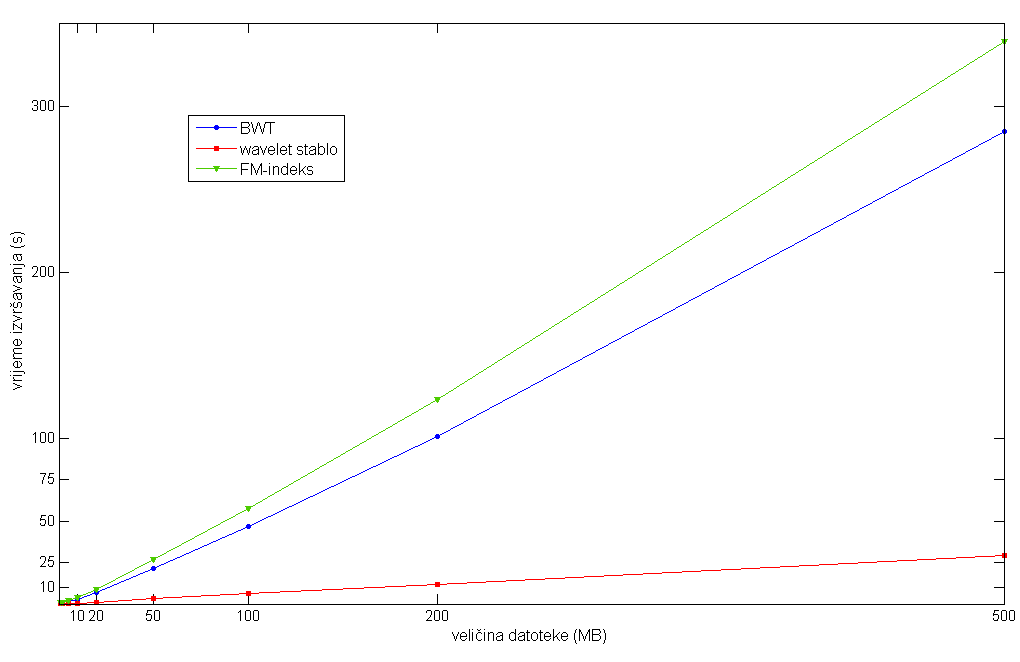
\includegraphics[width=\textwidth]{./pictures/test_nukl.png}
 \caption{Vremenska ovisnost trajanja algoritama o veličini datoteke koja sadrži nukleotide}
 \label{fig:test_nukl}
\end{figure}



Ukoliko malo proučimo podatke iz tablice i grafova, možemo vidjeti kako je složenost izgradnje indeksa linearno ovisna o veličini ulaznog niza. To je svojstvo koje smo i željeli postići, odnosno htjeli smo da nam je složenost izgradnje indeksa linearna. Iz priložene tablice i grafa vidimo kako je proces izgradnje FM-indeksa za veće ulazne datoteke veoma zahtjevan i dugotrajan proces, koji može potrajati i do nekoliko minuta. Upravo iz tog razloga javlja se potreba za pronalaskom što efikasnijih algoritama koji bi se mogli koristiti u postupku izgradnje FM-indeksa.

Pogledajmo sada vrijeme potrebno za izgradnju FM-indeksa nad proteinskim nizovima. U tablici \ref{tbl:tablProteini} prikazani su rezultati koji su dobiveni za datoteke koje su sadržavale proteinske nizove. Slika \ref{fig:test_proteini} prikazuje ovisnost izgradnje pojedinih dijelova FM-indeksa, kao i samog FM-indeksa u ovisnosti o veličini ulaznog niza, odnosno ulazne datoteke.


\begin{table}[H]
\caption{Testiranje na proteinima}
\label{tbl:tablProteini}
\centering
\begin{tabular}{c|c|c|c|}
\cline{2-4}
      	    					 & \multicolumn{3}{c|}{vrijeme izgradnje (s)}  \\ \hline
\multicolumn{1}{ |c| } {veličina (MB)} &	 BWT 	& wavelet stablo & FM indeks  \\ \hline 
\multicolumn{1}{ |c| } {   1    } 		& 	0.4547	&	0.366	&	0.9295	\\ \hline
\multicolumn{1}{ |c| } {   2    } 		& 	0.6815	&	0.4119	&	1.2776	\\ \hline
\multicolumn{1}{ |c| } {   5    } 		& 	1.5011	&	0.5886	&	2.5025	\\ \hline
\multicolumn{1}{ |c| } {   10    } 	&	3.2401	&	0.8957	&	4.9289	\\ \hline
\multicolumn{1}{ |c| } {   20    } 	&	7.392		&	1.4896	&	10.4347	\\ \hline
\multicolumn{1}{ |c| } {   50    } 	&	24.1723	&	4.61334	&	32.6025	\\ \hline
\multicolumn{1}{ |c| } {   100    } 	&	52.6474	&	7.7732	&	67.9625	\\ \hline
\multicolumn{1}{ |c| } {   200    } 	&	112.8949	&	13.9333	&	142.1054	\\ \hline
\multicolumn{1}{ |c| } {   500    } 	&	315.5526	&	32.8476	&	386.6631	\\ \hline
\end{tabular}
\end{table}


\begin{figure}[h]
   \centering
       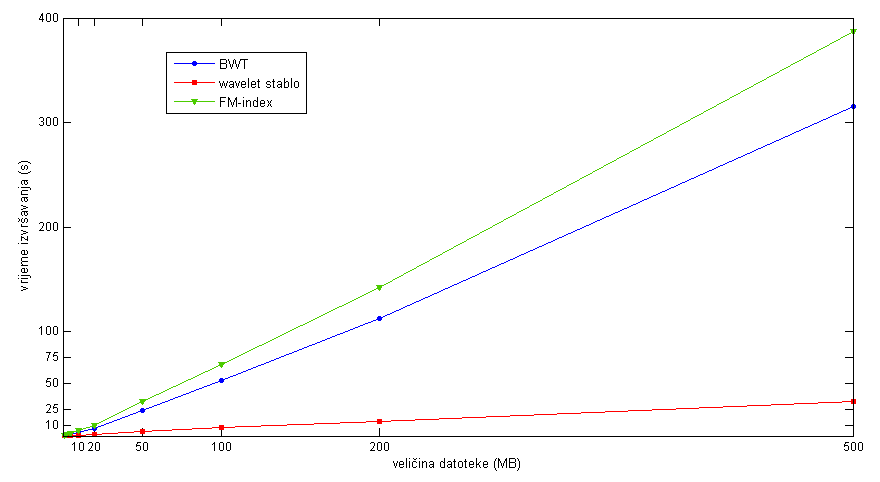
\includegraphics[width=\textwidth]{./pictures/test_proteini.png}
 \caption{Vremenska ovisnost trajanja algoritama o veličini datoteke koja sadrži proteine}
 \label{fig:test_proteini}
\end{figure}


Konačno, u tablici \ref{tbl:tablRand} je prikazana i ovisnost izgradnje FM-indeksa o veličini ulaznog niza za treću vrstu datoteka. Ovisnost izgradnje FM-indeksa, provođenja BWT transformacije, kao i izgradnju wavelet stabla, u odnosu na veličinu ulaznog niza prikazana je na slici \ref{fig:test_ascii}.


\begin{table}[H]
\caption{Testiranje na ASCII znakovima}
\label{tbl:tablRand}
\centering
\begin{tabular}{c|c|c|c|}
\cline{2-4}
      	    					 & \multicolumn{3}{c|}{vrijeme izgradnje (s)}  \\ \hline
\multicolumn{1}{ |c| } {veličina (MB)} & 	BWT 		& wavelet stablo & FM indeks  \\ \hline  
\multicolumn{1}{ |c| } {   1    } 		& 	0.4795	&	1.2554	&	1.9021	\\ \hline
\multicolumn{1}{ |c| } {   2    } 		& 	0.772	&	1.3382	&	2.4216	\\ \hline
\multicolumn{1}{ |c| } {   5    } 		& 	1.8199	&	1.789	&	4.34387	\\ \hline
\multicolumn{1}{ |c| } {   10    } 	&	4.2868	&	2.579	&	8.3161	\\ \hline
\multicolumn{1}{ |c| } {   20    } 	&	10.2298	&	4.061	&	17.1314	\\ \hline
\multicolumn{1}{ |c| } {   50    } 	&	31.4606	&	8.3703	&	46.9771	\\ \hline
\multicolumn{1}{ |c| } {   100    } 	&	72.435	&	15.4384	&	103.1664	\\ \hline
\multicolumn{1}{ |c| } {   200    } 	&	163.362	&	29.5337	&	223.3576	\\ \hline
\multicolumn{1}{ |c| } {   500    } 	&	447.88	&	66.3437	&	588.4351	\\ \hline
\end{tabular}
\end{table}


\begin{figure}[h]
   \centering
       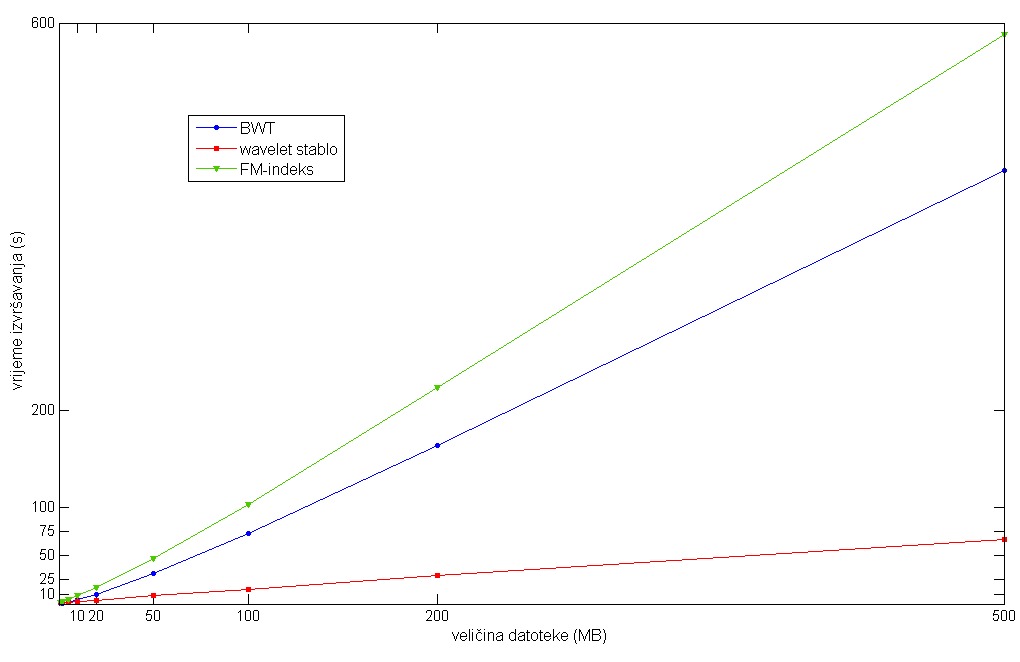
\includegraphics[width=\textwidth]{./pictures/test_ascii.png}
 \caption{Vremenska ovisnost trajanja algoritama o veličini datoteke koja sadrži ASCII znakove}
 \label{fig:test_ascii}
\end{figure}


Razmotrimo još za kraj ovog poglavlja vremenske ovisnosti izgradnje pojedinih struktura u ovisnosti o veličini ulazne datoteke, ali i o vrsti ulazne datoteke. Slike \ref{fig:test_bwt}, \ref{fig:test_wavelet}, \ref{fig:test_fm} prikazuju te ovisnosti za BWT transformaciju, izgradnju wavelet stabla i izgradnju FM-indeksa respektivno. Možemo vidjeti kako su za sve tri vrste datoteka te ovisnosti linearne za izgradnju svake od struktura (kao što je i prethodno bilo spomenuto). Također možemo vidjeti kako trajanje izgradnje indeksa ovisi o vrsti datoteke nad kojom se indeks izgrađuje. Iz slika se vidi kako se trajanje izgradnje indeksa za nizove nukleotida i proteina ne razlikuje jako puno, dok je vrijeme potrebno za izgradnju indeksa nad datotekama s ASCII znakovima značajno veće. Ukoliko se vratimo na tablicu \ref{tbl:alphabetsize} možemo vidjeti kako se ti nizovi razlikuju po veličini njihovih abeceda. Odatle možemo zaključiti kako trajanje izgradnje FM-indeksa uvelike ovisi i o veličini abecede nad kojom su ti nizovi izgrađeni, odnosno da će trajanje izgradnje biti veće što je veličina abecede ulaznog niza veća.


\begin{figure}[H]
   \centering
       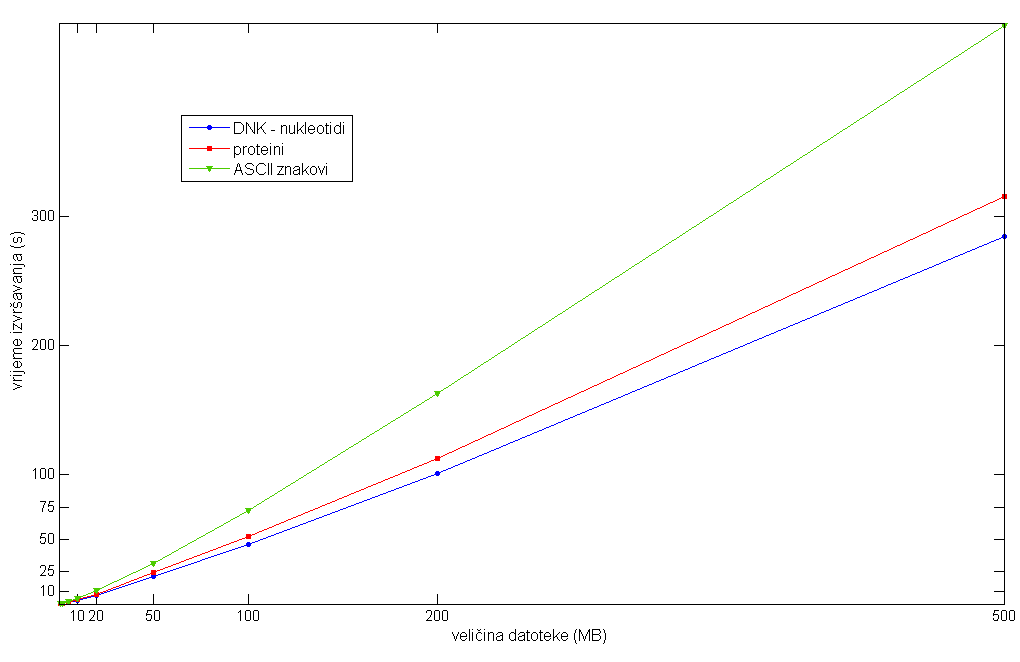
\includegraphics[width=\textwidth]{./pictures/test_bwt.png}
 \caption{Vremenska ovisnost trajanja BWT algoritma o veličini datoteke određenog tipa}
 \label{fig:test_bwt}
\end{figure}

\begin{figure}[H]
   \centering
       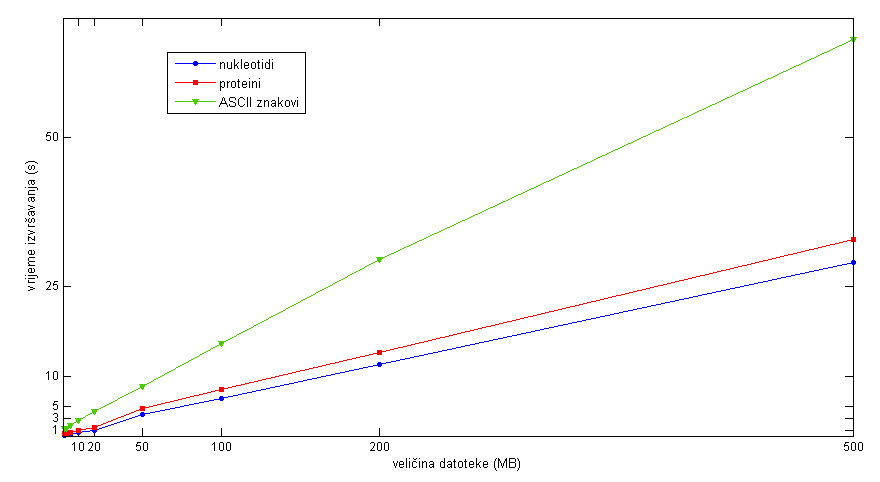
\includegraphics[width=\textwidth]{./pictures/test_wavelet.png}
 \caption{Vremenska ovisnost trajanja stvaranja wavelet stabla o veličini datoteke određenog tipa}
 \label{fig:test_wavelet}
\end{figure}

\begin{figure}[H]
   \centering
       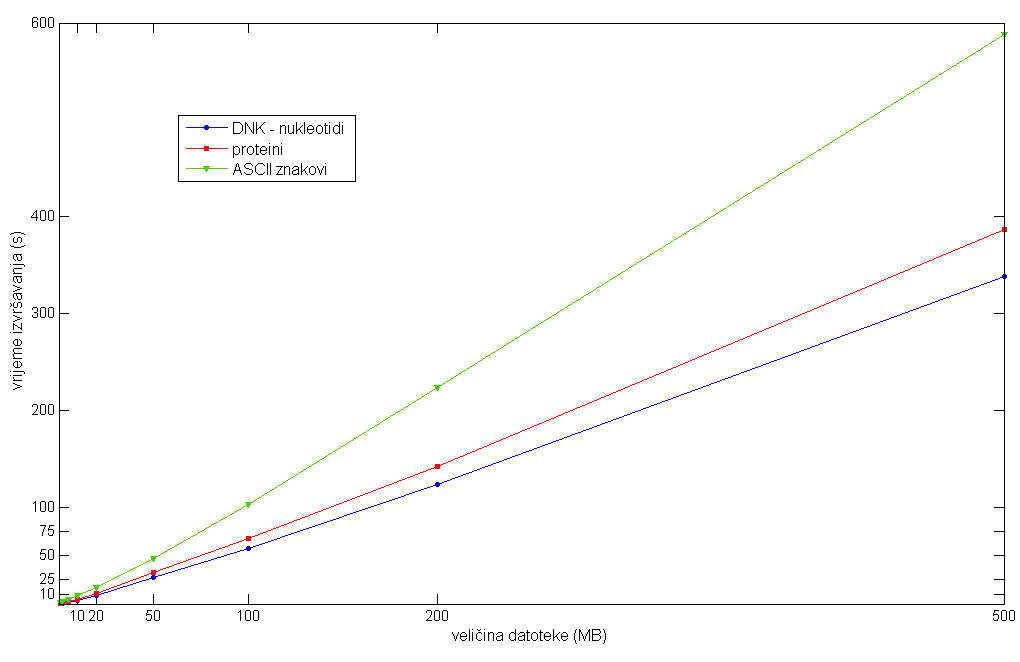
\includegraphics[width=\textwidth]{./pictures/test_fm.png}
 \caption{Vremenska ovisnost trajanja stvaranja FM-indeksa o veličini datoteke određenog tipa}
 \label{fig:test_fm}
\end{figure}




\section{Vrijeme obavljanja \textit{count} upita}

Drugi važan parametar pomoću kojeg se može ocijeniti uspješnost implementacije FM-indeksa jest obavljanje \textit{count} upita nad izgrađenim nizom. Dakle, sada kada je izgrađen FM-indeks želimo vidjeti koliko brzo se može izračunati pojavljivanje nekog podniza u nizu nad kojim je indeks izgrađen. Osim toga, želimo vidjeti i kako veličina niza nad kojim je izgrađen indeks utječe na trajanje prebrojavanja. Krenimo dakle redom. Tablice \ref{tbl:tablCountNukl}, \ref{tbl:tablCountProt} i \ref{tbl:tablCountRand} prikazuju trajanje prebrojavanja pojavljivanja nekog podniza u indeksu. Iz tablica se mogu izvesti neki veoma važni zaključci. Kao prvo, vidi se da trajanje prebrojavanja raste otprilike linearno s porastom duljine uzorka koji se traži. Nadalje, kroz sve tablice vidi se kako vrijeme prebrojavanja nekog uzorka ne ovisi o veličini ulaznog niza nad kojim je indeks izgrađen (u tablici \ref{tbl:tablCountNukl} se može uočiti jedna mala anomalija, odnosno skok u trajanju prebrojavanja između datoteke od 20MB i 50MB, no to je iz razloga što je uočeno kako u datoteci od 20MB i manje postoji samo 6 različitih znakova, dok u onima od 50MB naviše postoji 16 različitih znakova). Konačno, uspoređujući tablice možemo vidjeti kako trajanje obavljanja prebrojavanja ovisi o veličini abecede nad kojom je ulazni niz izgeneriran. To je iz razloga što se za obavljanje prebrojavanja koristi wavelet stablo čija veličina ovisi upravo o veličini abecede. 




\begin{table}[H]
\caption{\emph{count} upit nad DNK}
\label{tbl:tablCountNukl}
\centering
\begin{tabular}{c|c|c|c|c|c|c|}
\cline{2-7}
							& \multicolumn{6}{|c|}{trajanje prebrojavanja (ms)}  \\ \cline{2-7}  
      	    					 	& \multicolumn{6}{c|}{duljina traženog niza}  \\ \hline
\multicolumn{1}{ |c| } {veličina (MB)} & 100 & 200 & 300 & 400 & 500 & 1000	\\ \hline  
\multicolumn{1}{ |c| } {   1    } 		& 2 	& 3 	 & 5	    & 7	 & 8	 & 17		\\ \hline
\multicolumn{1}{ |c| } {   2    } 		& 2 	& 4	 & 5 	    & 7 	 & 7	 & 17 	\\ \hline
\multicolumn{1}{ |c| } {   5    } 		& 2 	& 3	 & 5	    & 7	 & 7	 & 16		\\ \hline
\multicolumn{1}{ |c| } {   10    } 	& 2 	& 3	 & 5	    & 7	 & 8	 & 16		\\ \hline
\multicolumn{1}{ |c| } {   20    } 	& 1	& 4	 & 5	    & 7	 & 8	 & 16		\\ \hline
\multicolumn{1}{ |c| } {   50    } 	& 2 	& 5	 & 7	    & 8	 & 10	 & 22		\\ \hline
\multicolumn{1}{ |c| } {   100    }	& 2 	& 4	 & 7	    & 8	 & 10 & 22		\\ \hline  
\multicolumn{1}{ |c| } {   200    }	& 2 	& 4	 & 7	    & 9	 & 9	 & 22		\\ \hline	
\multicolumn{1}{ |c| } {   500    } 	& 3 	& 4	 & 7	    & 7 	& 10	 & 23		\\ \hline
\end{tabular}
\end{table}



\begin{table}[H]
\caption{\emph{count} upit nad proteinima}
\label{tbl:tablCountProt}
\centering
\begin{tabular}{c|c|c|c|c|c|c|}
\cline{2-7}
							& \multicolumn{6}{|c|}{trajanje prebrojavanja (ms)}  \\ \cline{2-7}  
      	    					 	& \multicolumn{6}{c|}{duljina traženog niza}  \\ \hline
\multicolumn{1}{ |c| } {veličina (MB)} & 100 & 200 & 300 & 400 & 500 & 1000	\\ \hline  
\multicolumn{1}{ |c| } {   1    } 		& 3 	& 5    & 8	    & 9	& 9	 & 25		\\ \hline
\multicolumn{1}{ |c| } {   2    } 		& 3 	& 5	 & 8	    & 8 	& 10	 & 24		\\ \hline
\multicolumn{1}{ |c| } {   5    } 		& 3 	& 5	 & 7	    & 9	& 10	 & 23		\\ \hline
\multicolumn{1}{ |c| } {   10    } 	& 2 	& 5	 & 7	    & 8	& 10	 & 23		\\ \hline
\multicolumn{1}{ |c| } {   20    } 	& 2	& 5	 & 8	    & 9	& 11	 & 24		\\ \hline
\multicolumn{1}{ |c| } {   50    } 	& 2 	& 6	 & 8	    & 9	& 11	 & 26		\\ \hline
\multicolumn{1}{ |c| } {   100    }	& 2 	& 5	 & 9 	    & 9 	& 12	 & 24		\\ \hline  
\multicolumn{1}{ |c| } {   200    }	& 3 	& 5	 & 8	    & 9 	& 11	 & 25		\\ \hline	
\multicolumn{1}{ |c| } {   500    } 	& 3 	& 5	 & 7	    & 9	& 11	 & 24		\\ \hline
\end{tabular}
\end{table}


\begin{table}[H]
\caption{\emph{count} upit nad ASCII znakovima}
\label{tbl:tablCountRand}
\centering
\begin{tabular}{c|c|c|c|c|c|c|}
\cline{2-7}
							& \multicolumn{6}{|c|}{trajanje prebrojavanja (ms)}  \\ \cline{2-7}  
      	    					 	& \multicolumn{6}{c|}{duljina traženog niza}  \\ \hline
\multicolumn{1}{ |c| } {veličina (MB)} & 100 & 200 & 300 & 400 & 500 & 1000	\\ \hline 
\multicolumn{1}{ |c| } {   1    } 		& 3 	& 8 	 & 11	    & 13	& 18	 & 34		\\ \hline
\multicolumn{1}{ |c| } {   2    } 		& 4 	& 7	 & 11	    & 12 	& 18	 & 33		\\ \hline
\multicolumn{1}{ |c| } {   5    } 		& 4 	& 7	 & 10	    & 12	& 19	 & 34		\\ \hline
\multicolumn{1}{ |c| } {   10    } 	& 4 	& 8	 & 10	    & 13	& 19	 & 35		\\ \hline
\multicolumn{1}{ |c| } {   20    } 	& 4	& 8	 & 10	    & 12	& 19	 & 35		\\ \hline
\multicolumn{1}{ |c| } {   50    } 	& 4 	& 8	 & 11	    & 13 	& 19	 & 35		\\ \hline
\multicolumn{1}{ |c| } {   100    }	& 4 	& 8	 & 11	    & 14	& 20	 & 36		\\ \hline
\multicolumn{1}{ |c| } {   200    }	& 4 	& 8	 & 11	    & 13 	& 19	 & 38		\\ \hline
\multicolumn{1}{ |c| } {   500    } 	& 4 	& 8	 & 11	    & 13 	& 20	 & 36		\\ \hline
\end{tabular}
\end{table}

Potrebno je napomenuti kako izrada mjerenja u milisekundama naravno nije najbolja praksa, no nažalost ovako su ipak dobiveni najuvjerljiviji rezultati, jer je uočeno da prilikom obavljanja više uzastopnih upita dolazi do anomalije da se vremena obavljanja upita znaju smanjiti. Uzrok tomu je vjerojatno što se određeni podaci spreme u priručnu memoriju, pa se onda mogu puno brže dohvatiti prilikom ponovnog obavljanja prebrojavanja nekog niza.

Za kraj pogledajmo još sliku \ref{fig:test_count} na kojoj je prikazan graf gdje su iscrtane ovisnosti obavljanja prebrojavanja nekog uzorka u ovisnosti o duljini tog uzorka i u ovisnosti o veličini abecede niza nad kojim je izgrađen indeks (veličina datoteke nad kojom su se obavljali ovi eksperimenti bila je 500MB). Možemo vidjeti kako vrijeme prebrojavanja nekog uzorka raste  linearno s veličinom uzorka kojeg se pretražuje (što je već ranije u tekstu utvrđeno). Također se na ovom grafu lijepo može vidjeti kako je obavljanje prebrojavanja također ovisno i o veličini abecede niza nad kojim je indeks izgrađen.

\begin{figure}[H]
   \centering
       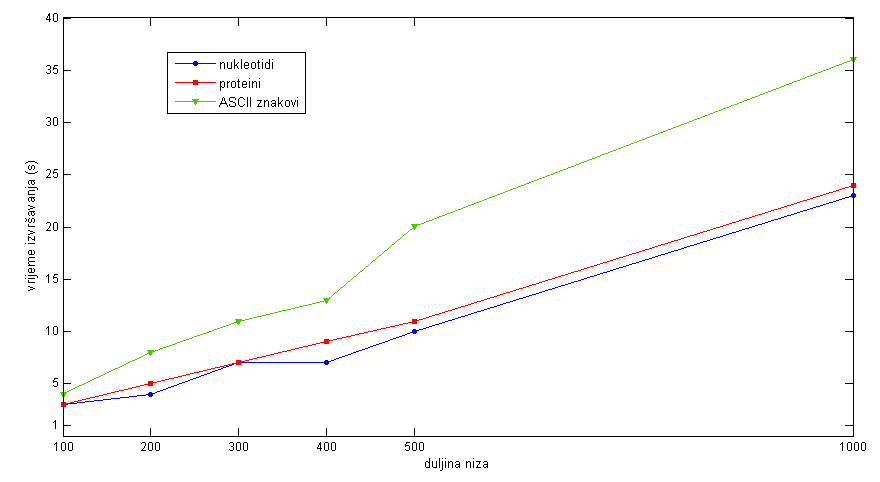
\includegraphics[width=\textwidth]{./pictures/test_count.png}
 \caption{Vremenska ovisnost izvršavanja \emph{count} algoritma o veličini niza koji se prebrojava}
 \label{fig:test_count}
\end{figure}


\section{Memorijsko zauzeće FM-indeksa}

Posljednji parametar kojeg možemo promatrati tijekom izrade FM-indeksa jest memorijsko zauzeće programa. U ovom poglavlju istaknut ćemo koliko je memorijsko zauzeće tokom izgradnje indeksa, kao i na kraju kada je indeks u potpunosti izgrađen. Osim toga, u ovom poglavlju pokazat će se kako Java virtualni stroj zauzima mnogo više memorije nego što je zaista potrebno za samo izvođenje algoritma, što predstavlja jedan veliki nedostatak. Ovdje će se razmotriti memorijska zauzeća za sve tipove datoteka, no promatrat će se samo veličine datoteka od 50MB nadalje. U tablicama \ref{tbl:tablMemNukl}, \ref{tbl:tablMemProt} i \ref{tbl:tablMemRand} je prikazana potrošnja memorije FM-indeksa za sve tri vrste datoteka i različite veličine datoteka. Izdvojena su tri stupca u tablicama, od kojih prvi stupac predstavlja maksimalnu memoriju koju je cijeli proces zauzeo. Drugi stupac predstavlja maksimalnu količinu memorije koju je algoritam u nekom trenutku koristio, dok treći stupac predstavlja stvarno zauzeće memorije (dakle količinu memorije koju stvarno zauzimaju izgrađene strukture) od strane izgrađenog indeksa. Iz tablica se vidi kako je maksimalna memorija koja je zauzeta od strane Java virtualnog stroja puno veća nego li je za rad algoritma potrebno. To je ogroman nedostatak, jer ispada da su memorijski zahtjevi mnogo veći nego što oni uistinu jesu.


\begin{table}[h]
\caption{Memorijsko zauzeće - DNK}
\label{tbl:tablMemNukl}
\centering
\begin{tabular}{c|c|c|c|}
\cline{2-4}
      	   & \multicolumn{3}{c|}{memorijsko zauzeće (MB)}  \\ \hline
\multicolumn{1}{ |c| } {veličina (MB)} & maksimalno & pravo & konačno  \\ \hline
\multicolumn{1}{ |c| } {   50   }		&	393	&	314	&	53	\\ \hline
\multicolumn{1}{ |c| } {  100  }		&	803	&	620	&	103	\\ \hline
\multicolumn{1}{ |c| } {  200  }		&	1553	&	1230	&	201	\\ \hline
\multicolumn{1}{ |c| } {  500   } 	&	3830	&	3080	&	494	\\ \hline
\end{tabular}
\end{table}



\begin{table}[h]
\caption{Memorijsko zauzeće - proteini}
\label{tbl:tablMemProt}
\centering
\begin{tabular}{c|c|c|c|}
\cline{2-4}
      	   & \multicolumn{3}{c|}{memorijsko zauzeće (MB)}  \\ \hline
\multicolumn{1}{ |c| } {veličina (MB)} & maksimalno & pravo & konačno  \\ \hline
\multicolumn{1}{ |c| } {   50   }		&	370	&	292	&	67	\\ \hline
\multicolumn{1}{ |c| } {   100   }	&	800	&	614	&	130	\\ \hline
\multicolumn{1}{ |c| } {   200   }	&	1550	&	1230	&	254	\\ \hline
\multicolumn{1}{ |c| } {   500   }	&	4800	&	3070	&	680	\\ \hline
\end{tabular}
\end{table}


\begin{table}[h]
\caption{Memorijsko zauzeće - ASCII znakovi}
\label{tbl:tablMemRand}
\centering\begin{tabular}{c|c|c|c|}
\cline{2-4}
      	   & \multicolumn{3}{c|}{memorijsko zauzeće (MB)}  \\ \hline
\multicolumn{1}{ |c| } {veličina (MB)} & maksimalno & pravo & konačno  \\ \hline
\multicolumn{1}{ |c| } {   50   }		&	432	&	365	&	100	\\ \hline
\multicolumn{1}{ |c| } {   100   }	&	800	&	619	&	191	\\ \hline
\multicolumn{1}{ |c| } {   200   }	&	1558	&	1235	&	378	\\ \hline
\multicolumn{1}{ |c| } {   500   }	&	4000	&	3700	&	840	\\ \hline
\end{tabular}
\end{table}

Slike \ref{fig:test_mem_nukl}, \ref{fig:test_mem_proteini} i \ref{fig:test_mem_ascii} prikazuju grafičke prikaze prethodno navedenih tablica radi boljeg pregleda. Iz tablica i slika se može vidjeti kako prosječno memorijsko zauzeće izgradnje FM-indeksa za sve inačice iznosi otprilike $6n$ (ovdje se misli na memoriju koju algoritam stvarno koristi) pri čemu je $n$ veličina ulaznog niza. U tablici \ref{fig:test_mem_ascii} se može vidjeti kako je u 2 slučaja bilo potrebno i nešto više memorije od toga. Razlog tome nije direktno poznat, no vjerojatno se radi o većem broju rekurzivnih poziva prilikom konstrukcije sufiksnog polje, jer se u tom postupku koriste dodatne strukture koje mogu povećati memorijsku potrošnju. Osim toga, te su datoteke izgenerirane u potpunosti nasumično, bez ikakvih pravilnosti i nad većim abecedama. Vidimo da se kod ostalih datoteka algoritam ponaša očekivano. Nakon izgradnje vidimo da FM-indeks zauzima mnogo manje memorija nego je bilo potrebno za izgradnju. Koliko točno memorije će zauzimat će opet ovisiti o tome kolika je veličina abecede nad kojom je indeks izgrađen. Vidimo da za nukleotidne nizove FM-indeks zauzima otprilike istu količinu memorije kao i originalni niz. Kako se veličina abecede povećava, tako se i povećava količina memorije koju FM-indeks zauzima nakon izgradnje.


\begin{figure}[H]
   \centering
       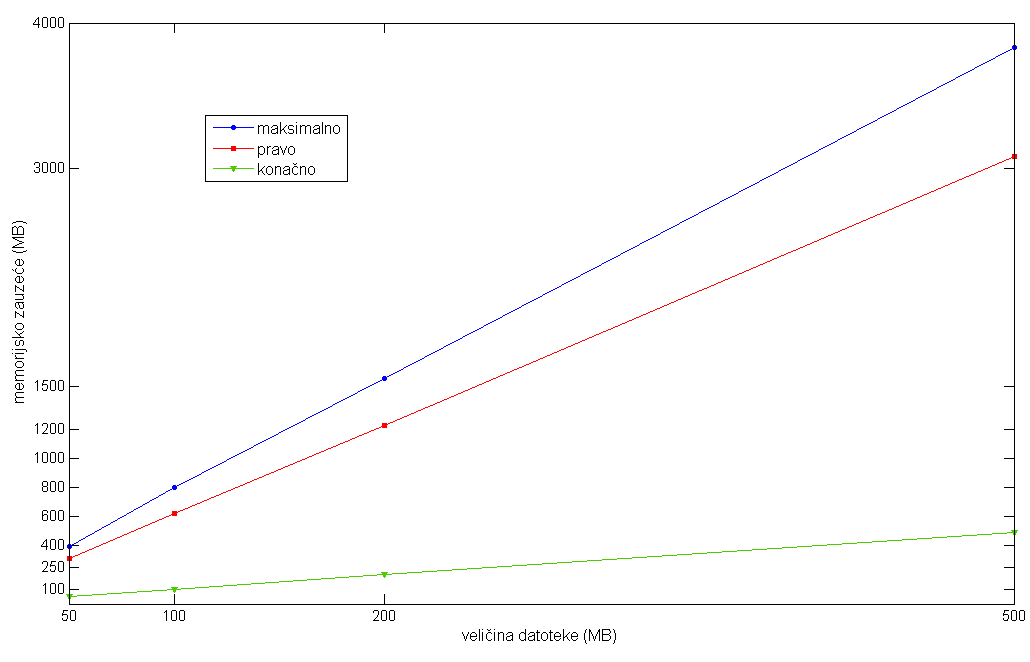
\includegraphics[width=\textwidth]{./pictures/test_mem_nukl.png}
 \caption{Memorijska ovisnost stvaranja FM-indeksa algoritama o veličini datoteke koja sadrži nukleotide}
 \label{fig:test_mem_nukl}
\end{figure}

\begin{figure}[H]
   \centering
       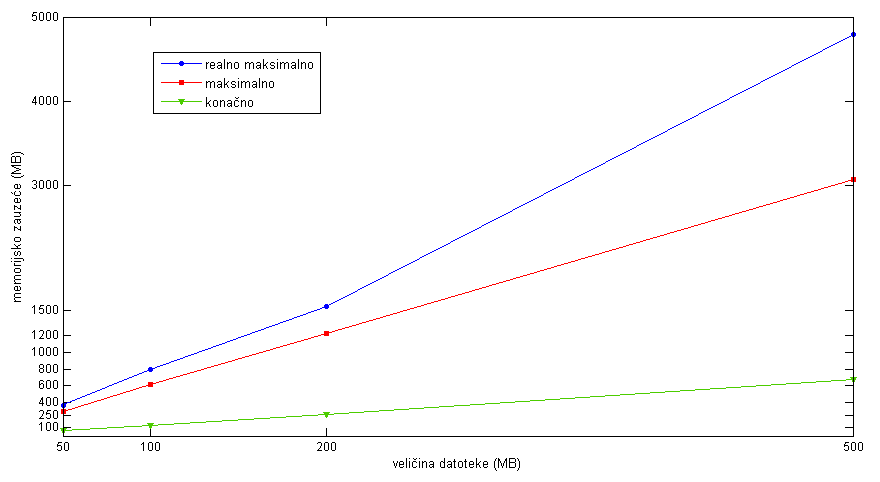
\includegraphics[width=\textwidth]{./pictures/test_mem_proteini.png}
 \caption{Memorijska ovisnost stvaranja FM-indeksa algoritama o veličini datoteke koja sadrži proteine}
 \label{fig:test_mem_proteini}
\end{figure}

\begin{figure}[H]
   \centering
       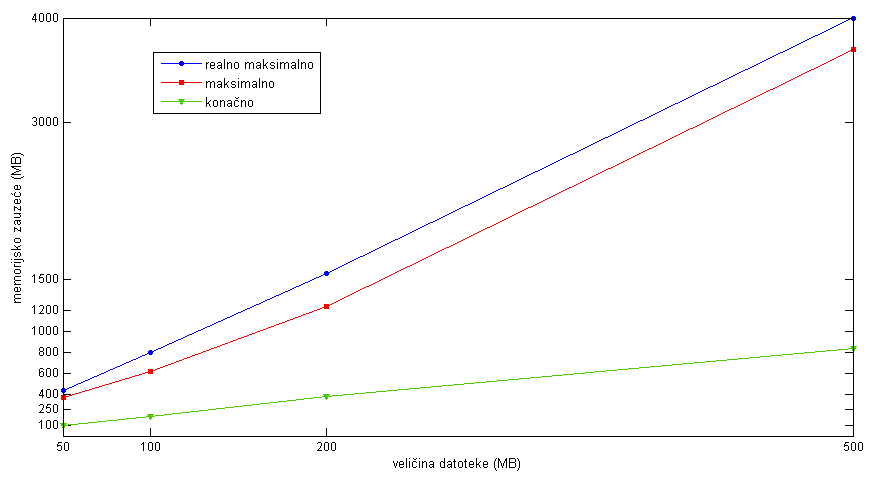
\includegraphics[width=\textwidth]{./pictures/test_mem_ascii.png}
 \caption{Memorijska ovisnost stvaranja FM-indeksa algoritama o veličini datoteke koja sadrži ASCII znakove}
 \label{fig:test_mem_ascii}
\end{figure}

Slika  \ref{fig:test_mem_pravo} prikazuje maksimalnu memorijsku potrošnju algoritma. Ovo je zapravo veličina koja nas najviše zanima. Vidimo kako je memorijska potrošnja za sve datoteke u istim veličinama gotovo podjednaka (osim onih dviju datoteka koje ponešto odstupaju). Vidimo kako se algoritam ponaša veoma poželjno i kako otprilike znamo koliku memorijsku potrošnju možemo očekivati s obzirom na ulazni niz.

\begin{figure}[H]
   \centering
       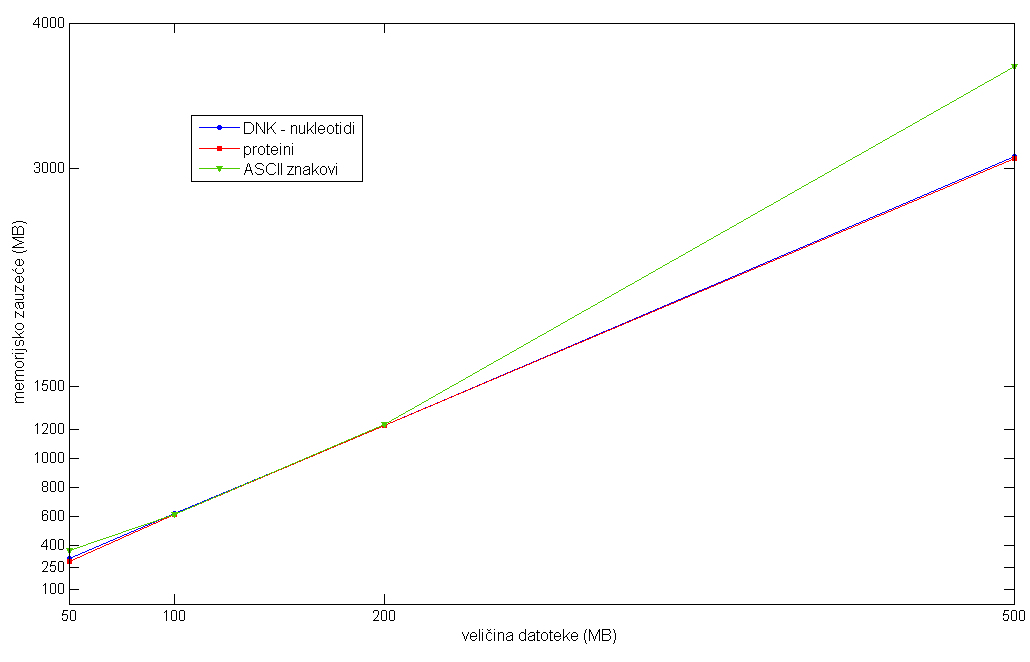
\includegraphics[width=\textwidth]{./pictures/test_mem_pravo.png}
 \caption{Memorijska (maksimalna) ovisnost stvaranja FM-indeksa o veličini datoteke određenog tipa}
 \label{fig:test_mem_pravo}
\end{figure}

Slika \ref{fig:test_mem_max} prikazuje maksimalnu memoriju koju je program zauzeo tijekom izgradnje indeksa za svaki tip datoteke po različitim veličinama. Ovaj graf se neće posebno komentirati jer on zapravo ni ne predstavlja pravu memorijsku potrošnju algoritma.


\begin{figure}[H]
   \centering
       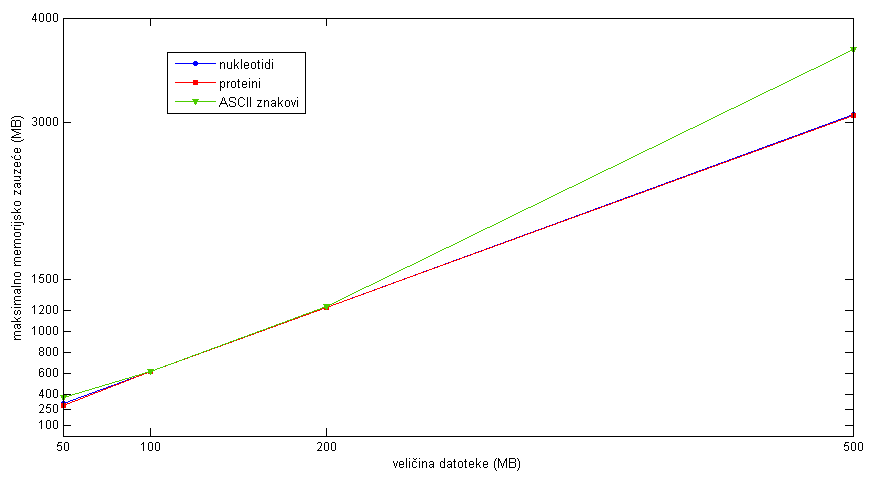
\includegraphics[width=\textwidth]{./pictures/test_mem_max.png}
 \caption{Memorijska (realno maksimalna) ovisnost stvaranja FM-indeksa o veličini datoteke određenog tipa}
 \label{fig:test_mem_max}
\end{figure}

Slika \ref{fig:test_mem_kon} prikazuje memorijska zauzeća FM-indeksa nakon što je izgrađen. Vidi se kako to zauzeće ovisi o ulaznom nizu, ali ne samo to, ono ovisi i o veličini abecede ulaznog niza. Što je abeceda manja to će i zauzeće indeksa biti manje.

\begin{figure}[H]
   \centering
       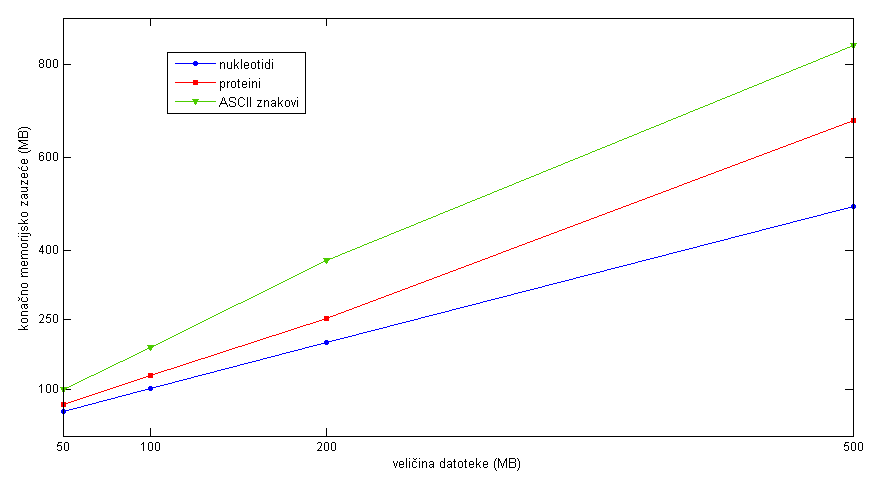
\includegraphics[width=\textwidth]{./pictures/test_mem_kon.png}
 \caption{Memorijska (konačna) ovisnost stvaranja FM-indeksa o veličini datoteke određenog tipa}
 \label{fig:test_mem_kon}
\end{figure}




Pogledajmo sada sliku \ref{fig:profiler}, preuzetu iz alata Jprofiler, koje predstavlja memorijsko zauzeće algoritma kroz vrijeme. Plavom bojom označena je memorija koju program, odnosno algoritam stvarno koristi za spremanje struktura, dok je zelenom bojom označena slobodna memorija koju je Java virtualni stroj dodatno zauzeo. Vidimo da cijelo vrijeme Java virtualni stroj zauzima mnogo više memorije nego što mu doista treba za rad. To je ogroman nedostatak pri izradi memorijski zahtjevnih algoritama kao što je ovaj, jer Java programski jezik ne omogućuje efikasno rukovanje memorijom. Stoga je prilikom korištenja ovog programa potrebno imati na umu kako će realno zauzeće memorije zapravo biti veće od onog što algoritam zaista koristi.

\begin{figure}[H]
   \centering
       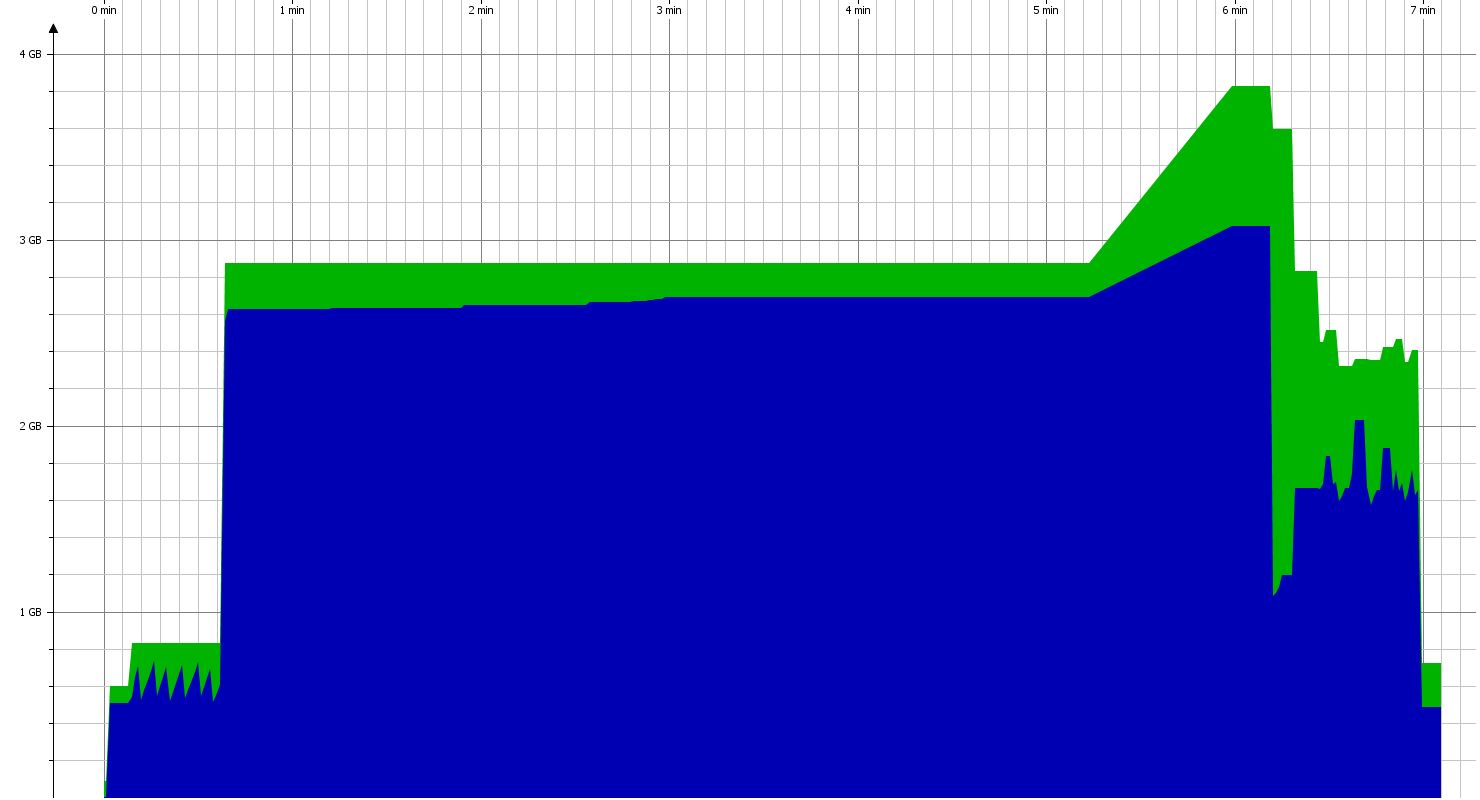
\includegraphics[width=\linewidth]{./pictures/profiler.jpg}
 \caption{Zauzeće memorije Java virtualnog stroja tijekom konstrukcije indeksa}
 \label{fig:profiler}
\end{figure}